\documentclass[
%   draft,
  a4paper,
%   titlepage,
  onecolumn,
%  twocolumn,
  11pt,
  ]%
% {scrartcl}%
{article}%


\usepackage[utf8x]{inputenc} 
%\usepackage[utf8]{inputenc} % codificação deste ficheiro em UTF-8 

\usepackage[T1]{fontenc} % necessário para que os caracteres acentuados possam ser considerados como um só bloco ( efeito colaterar: necessita de uma fonte que não a CM para não ficar com um aspecto aceitável)

%% precisa ser carregado um outro tipo de letra por causa do efeito colateral do pacote T1:
\usepackage{lmodern} % Fonte "Latin Modern" - A solução óptima para fontes latinas (resolve o problema do T1)
% \usepackage{times}   % Fonte "Times"


\usepackage{textcomp} % caracteres extra - símbolo do euro por exemplo

% \usepackage[portuguese]{babel} % tradução portuguesa
% \newcommand{\referencesname}{Bibliografia}
\newcommand{\referencesname}{References}


%%%%%%%%%% Packages


\usepackage[pdftex]{graphicx} % figuras 
% \usepackage{subfigure} % subfiguras ( a,b,... )
% \usepackage{wrapfig} % figuras ao lado de texto


\usepackage{array} % mais opções nas tabelas (m{width}, b{width}, ...)
\setlength{\extrarowheight}{1pt} % extra espaço entre as linhas das tabelas
% \usepackage{multirow} % tabelas com células multilinha

\usepackage{fancyhdr} % Estilo de página

% \usepackage{listings} % Highlight de código fonte
% \renewcommand{\lstlistingname}{Listagem} % tradução para português (referente ao package listings)
% \renewcommand{\lstlistlistingname}{Listagens} % tradução para português (referente ao package listings)

\usepackage[usenames,hyperref,pdftex%
 ,svgnames%
 ,x11names%
 ,dvipsnames%
%  ,cmyk
 ]{xcolor} % Utilização de cores
\usepackage{multicol}


\usepackage[left=2.3cm,right=2.3cm,top=2.4cm]{geometry} % Margins

% \usepackage{setspace} % spacing between lines (\singlespacing, \onehalfspacing, ...)

% math packages by AMS
\usepackage{amsmath} % main one
% \usepackage{amsfonts}
% \usepackage{amssymb}


% \usepackage{moreverb} % more verbatim options (boxedverbatim)
\usepackage{fancyvrb} % more verbatim options 

% \usepackage{lipsum}


% \usepackage{tikz}
% Optional tikz libraries
% \usetikzlibrary{arrows}
\usepackage{listings}
\lstset{language=Matlab,%
    %basicstyle=\color{red},
    breaklines=true,%
    morekeywords={matlab2tikz},
    keywordstyle=\color{blue},%
    morekeywords=[2]{1}, keywordstyle=[2]{\color{black}},
    identifierstyle=\color{black},%
    stringstyle=\color{mylilas},
    commentstyle=\color{mygreen},%
    showstringspaces=false,%without this there will be a symbol in the places where there is a space
    numbers=left,%
    numberstyle={\tiny \color{black}},% size of the numbers
    numbersep=9pt, % this defines how far the numbers are from the text
    emph=[1]{for,end,break},emphstyle=[1]\color{red}, %some words to emphasise
    %emph=[2]{word1,word2}, emphstyle=[2]{style},    
}


\usepackage[square, comma, sort&compress]{natbib}

\setcitestyle{super,comma}

% \usepackage[protrusion=true,expansion=true]{microtype}
\usepackage[protrusion=true,expansion=true,stretch=10,shrink=10]{microtype} % micro-typographic extensions of pdfTEX (gets high quality text compostion)

\usepackage[
      pdftex,             %driver
      colorlinks=true,    %no frame around URL
      urlcolor=DarkGreen!70!Black,    %no colors
%       menucolor=black,    %no colors
      linkcolor=black,    %no colors
%       pagecolor=black,    %no colors
      citecolor=DarkGreen!70!Black,    %no colors
      bookmarks=true,    %tree-like TOC
      bookmarksopen=true,    %expanded when starting
      bookmarksnumbered=true, %Put section numbers in bookmarks
      hyperfootnotes=true,    %no referencing of footnotes, does not compile
      pdfpagemode=UseOutlines,    %show the bookmarks when starting the pdf viewer
      plainpages=false, %solve problem ``destination with the same identifier'' warning
      pdfpagelabels %solve problem ``destination with the same identifier'' warning
]{hyperref} % fazer hyperlinks (usar como último ``usepackage'')


% \usepackage[style=altlist,hypertoc,hyper,number=page]{glossary}


% \usepackage{pdfpages}

 \usepackage[]{todonotes}
% \usepackage[disable]{todonotes}

\usepackage{xifthen}
\usepackage{csvsimple}



\newcommand{\tab}{\hspace*{2em}}

%Text subscript
\usepackage{fixltx2e}

% Matrizes
\usepackage{amsmath}

%rename defaults




%Figure side by side

\usepackage{subfig}

%force float position
\usepackage{float}
\usepackage[section]{placeins}

\makeatletter
\AtBeginDocument{%
  \expandafter\renewcommand\expandafter\subsection\expandafter{%
    \expandafter\@fb@secFB\subsection
  }%
}
\makeatother
%%%%%%%%%%%%%%%%%%%%%%%%%%%%%%%%%%%%%%%%%%%%%%%%%%%%%%%%%%%%%%%% 


% Ifenização
%\hyphenation{apli-ca-ção cons-tru-ção}% ...

%%%%%%%%%%%%%%%%%%%%%%%%%%%%%%%%%%%%%%%%%%%%%%%%%%%%%%%%%%%%%%%%
%Parametros de exibicao de codigo
\usepackage{listings}
\usepackage{color}

\definecolor{mygreen}{rgb}{0,0.6,0}
\definecolor{mygray}{rgb}{0.5,0.5,0.5}
\definecolor{mymauve}{rgb}{0.58,0,0.82}

\lstset{ %
  backgroundcolor=\color{white},   % choose the background color; you must add \usepackage{color} or \usepackage{xcolor}
  basicstyle=\footnotesize,        % the size of the fonts that are used for the code
  breakatwhitespace=false,         % sets if automatic breaks should only happen at whitespace
  breaklines=true,                 % sets automatic line breaking
  captionpos=b,                    % sets the caption-position to bottom
  commentstyle=\color{mygreen},    % comment style
  deletekeywords={...},            % if you want to delete keywords from the given language
  escapeinside={\%*}{*)},          % if you want to add LaTeX within your code
  extendedchars=true,              % lets you use non-ASCII characters; for 8-bits encodings only, does not work with UTF-8
  frame=single,                    % adds a frame around the code
  keepspaces=true,                 % keeps spaces in text, useful for keeping indentation of code (possibly needs columns=flexible)
  keywordstyle=\color{blue},       % keyword style
  language=Matlab,                 % the language of the code
  morekeywords={*,...},            % if you want to add more keywords to the set
  numbers=left,                    % where to put the line-numbers; possible values are (none, left, right)
  numbersep=5pt,                   % how far the line-numbers are from the code
  numberstyle=\tiny\color{mygray}, % the style that is used for the line-numbers
  rulecolor=\color{black},         % if not set, the frame-color may be changed on line-breaks within not-black text (e.g. comments (green here))
  showspaces=false,                % show spaces everywhere adding particular underscores; it overrides 'showstringspaces'
  showstringspaces=false,          % underline spaces within strings only
  showtabs=false,                  % show tabs within strings adding particular underscores
  stepnumber=2,                    % the step between two line-numbers. If it's 1, each line will be numbered
  stringstyle=\color{mymauve},     % string literal style
  tabsize=2,                       % sets default tabsize to 2 spaces
  title=\lstname                   % show the filename of files included with \lstinputlisting; also try caption instead of title
  %inputencoding=ansinew
}


%%%%%%%%%%%%%%%%%%%%%%%%%%%%%%%%%%%%%%%%%%%%%%%%%%%%%%%%%%%%%%%%

%% Criação de comandos:


\newcommand{\note}[1]{{\sffamily \slshape \textcolor{red}{#1}}}

\colorlet{FPathColor}{Sepia}
\colorlet{CmdColor}{blue}
\colorlet{CmdRuleColor}{LightSteelBlue}
\colorlet{FileTextColor}{DarkGreen}
\colorlet{FuncColor}{DeepPink4}
\CustomVerbatimCommand{\FPath}{Verb}{formatcom=\color{FPathColor},fontsize=\normalsize}
\CustomVerbatimCommand{\Cmd}{Verb}{formatcom=\color{CmdColor},fontsize=\normalsize}
\CustomVerbatimCommand{\FText}{Verb}{formatcom=\color{FileTextColor},fontsize=\normalsize}
\CustomVerbatimCommand{\Func}{Verb}{formatcom=\color{FuncColor},fontsize=\normalsize}
\DefineVerbatimEnvironment%
  {Command}{Verbatim}
  {formatcom=\color{CmdColor},frame=single,rulecolor=\color{CmdRuleColor},fontsize=\normalsize}
\DefineVerbatimEnvironment%
  {FileText}{Verbatim}
  {formatcom=\color{FileTextColor},fontsize=\normalsize}


% % Authors:



\newcommand{\MYauthor}{José Pedro Medeiros}
\newcommand{\MYnumber}{2010129934} 


%\newcommand{\MYauthorIII}{------ ----- ----} 
%\newcommand{\MYnumberIII}{xxxxxxxxxx}



% % Titles:
\newcommand{\MYtitle}{Movement Generalization and Classification}
\newcommand{\MYsubtitle}{Kinesthetic Learning} % Can be empty


% % Course

\newcommand{\MYcoursename}{Learning by Demonstration applied to NAO Robot }
\newcommand{\MYcourseyear}{ 2015-2016 }


% % PDF infos

\newcommand{\MYkeywords}{} % Can be empty
\newcommand{\MYsubject}{} % Can be empty


%% Document format

%% Fancy Headers
\lhead{
\includegraphics[width=2cm]{logo_deec.pdf}}
\chead{\sc\footnotesize Universidade de Coimbra\\
Faculdade de Ciências e Tecnologia\\
Departamento de Engenharia Electrotécnica e de Computadores}
\rhead{
\includegraphics[width=0.8cm]{logo_fctuc.pdf}}
\setlength{\headheight}{43pt}

% Title
\title{{\large\MYcoursename\ -- \MYcourseyear}\\[2mm]
{\MYtitle}
\ifthenelse{\equal{\MYsubtitle}{}}
{\vspace*{1mm}}   {\\{\large\MYsubtitle}\vspace*{1mm}}
}

% Author / Number
\author{%
\MYauthor\\{\normalsize \href{mailto:ze_pedrom@hotmail.com}{\MYnumber}}
\ifthenelse{\isnamedefined{MYauthorII}}
{\and\MYauthorII\\{\normalsize \href{mailto:luis.rocha.jacinto@gmail.com}{\MYnumberII}}}    {}
\ifthenelse{\isnamedefined{MYauthorIII}}
{\and\MYauthorIII\\{\normalsize \href{mailto:a\MYnumberIII@alunos.deec.uc.pt}{\MYnumberIII}}}   {}
}

% Version / Date
\date{%
% \normalsize \today
\mbox{}
}




%% PDF definitions:

\hypersetup{%
   pdftitle=\MYtitle,%
   pdfauthor=\MYauthor,%
%    pdfcreator=,%
   pdfkeywords= {\MYkeywords},%
%    pdfproducer=,%
   pdfsubject= \MYsubject%
} % informações do pdf (pacote hyperref)

\pdfinfo{
/Title	(\MYtitle)
/Author (\MYauthor)
/Keywords (\MYkeywords)
} % informações do pdf

\graphicspath{ {img/} } % Pasta das Imagens










\begin{document}

\maketitle
\thispagestyle{fancyplain}

\setlength{\parskip}{10pt}
% Introdução
 \begin{abstract} % (optional)
 
This report describes four approaches for learning and generalize NAO Robot movements.
\indent All of the approaches are based on \cite{Calinon07}, where kinesthetic movements are learned and generalized by a robot. We have acquired a dataset consisting of data from 12 joints from NAO arms (6 joints
corresponding to the left arm and 6 joints corresponding to the right arm) in order to test it in the different approaches. This dataset was collected by reproducing the same movement on a total of 6 repetitions done by two different persons,
3 repetitions each.\\
\indent The approaches taken in this work have the goal to learn and represent a dataset of movements performed by the NAO robot trough kinesthetic  movements. In the first approach applied Principal Component Analysis \textbf{(PCA)} was used to reduce the dataset dimensions, later on the data was aligned using the Dynamic Time Warping \textbf{(DTW)}. These are two pre-processing steps
used to improve the Gaussian Mixture Model \textbf{(GMM)} algorithm that was applied to the resulting
data, next and finally after this classification we obtain a "signature" using the Gaussian Mixture
Regression \textbf{(GMR)}.\\
\indent In a second approach \textbf{GMM} and \textbf{GMR} were applied directly to the original data without any pre-processing steps.\\
\indent In the third approach the first two steps are equal to the first approach but instead of
concatenating the data, "signatures" were created for each repetition of the movement and in
the end, an average from all signatures was generated.\\
\indent The last approach applies \textbf{DTW} as a pre-processing step and \textbf{GMM} and \textbf{GMR} are applied in the concatenated data.
 
 \begin{figure}[ht]
\centering
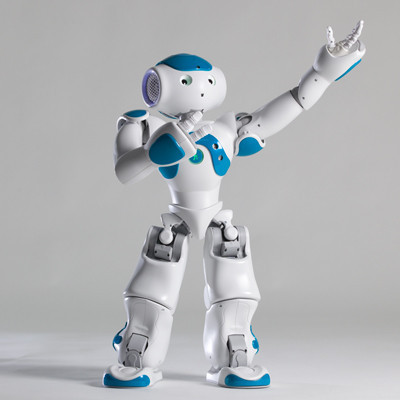
\includegraphics[width=60mm,scale=1]{1.jpg}
\caption{Imagem original}\label{fig:Nao}
\end{figure}
 \end{abstract}

\newpage





\tableofcontents

\section{Introduction}

\indent \\ \indent     The objective of this work is to learn, generalize and classify NAO robot movements. The kinesthetic movements were learned by NAO robot, the dataset was generated by repeating the same movement 6 times by two different persons, each person repeated the same movement 3 times. The robot learned 3 different movements, the "goodbye" movement, the "clapping" movement and the "bolt" movement. Since the 3 different movements only involved moving the arms, we focused on collecting the data related to the joints from the arms. NAO robot as 6 joints in each arm, so in total  we collected data from 12 different joints.\\
\indent For the data collection a python script was created. The script was programmed to read joint's values each 100 milliseconds, in the end it's created a .txt file containing data formatted in 12 vectors, each vector corresponding to one joint. Taking into account the time step time vectors were created for each vector. \\ \indent After this step, 4 different approaches were followed in order to generalize and classify the movements. All of these approaches were based on \cite{Calinon07}, section 3 of this report will explain in detail each one.\\ \indent Is important to refer that this report only present results for the "bolt" movement.



\section{Algorithms}
\subsection{Principal Component Analysis:}
Principal Component Analysis algorithm was applied to reduce the dataset dimension. Although we are not explaining here the algorithm in detail a brief explanation is given since it is important to understand how to approximate the data back to the original after \textbf{PCA} was applied. \\
If we start with a dataset $X_n^m$


\section*{Matlab Code}
(Melhorar)

[COEFF, PC, LATENT]  = pca(X);
 The combination pc * w' will recreate the original data, minus its mean.
 The mean is always subtracted prior to performing PCA. Therefore to get 
 the original data we do
mu = mean(X);
xhat = bsxfun(@minus,X,mu); % subtract the mean
norm(PC * COEFF' - xhat);


Because COEFF is orthogonal, you also have Xhat * COEFF = pc, 
 or schematically (i.e. this code won't execute) 
 (X - mu) * COEFF = PC     <=>      X = mu + PC * COEFF'


 To get an approximation to your original data, you can start dropping 
columns from the computed principal components. To get an idea of which
 columns to drop, we examine the LATENT( eigenvalues)
 Relevance=ev/sum(ev)*100


%Xapprox = PC(:,1:2) * COEFF(:,1:2)';
%Xapprox = bsxfun(@plus,mu,Xapprox); % add the mean back in
\subsection{Dynamic Time Warping:}
 
\subsection{Gaussian Mixture Model:}

\subsection{Gaussian Mixture Regression:}



\section{Approaches}
\subsection{First Approach:}
Given the movement observations represented in 2 dimensions vectors with raw data, time and joint values([-2;2]) , we have resized all vectors to the smallest sized one (if we resized to any other we could break or slow down the robot movements). After this step Principal Component Analysis \textbf{(PCA)} was applied to the vectors in order to reduce dimensionality of the data, as shown in \ref{my-label}.
      


\begin{table}[]
\centering
\caption{PCA Analysis}
\label{my-label}
\begin{tabular}{lcc}
\multicolumn{1}{c}{\textbf{Bolt Movement :}}                  & \textbf{Performance}                        & \multicolumn{1}{l}{\textbf{Number of Princ. Comp.}} \\ \hline
\multicolumn{1}{|l|}{Dataset: medeiros-bolt2015-12-7-17-4-31} & \multicolumn{1}{c|}{performance1 = 99.4579} & \multicolumn{1}{c|}{num\_pc1 = 3}                   \\ \hline
\multicolumn{1}{|l|}{Dataset: medeiros-bolt2015-12-7-17-5-12} & \multicolumn{1}{c|}{performance2 = 99.3659} & \multicolumn{1}{c|}{num\_pc2 = 3}                   \\ \hline
\multicolumn{1}{|l|}{Dataset: medeiros-bolt2015-12-7-17-5-12} & \multicolumn{1}{c|}{performance3 = 99.5385} & \multicolumn{1}{c|}{num\_pc3 = 4}                   \\ \hline
\multicolumn{1}{|l|}{Dataset:rui-bolt2015-12-7-17-5-49}       & \multicolumn{1}{c|}{performance4 = 99.4232} & \multicolumn{1}{c|}{num\_pc4 = 3}                   \\ \hline
\multicolumn{1}{|l|}{Dataset:rui-bolt2015-12-7-17-6-3}        & \multicolumn{1}{c|}{performance5 =99.0995}  & \multicolumn{1}{c|}{num\_pc5 = 2}                   \\ \hline
\multicolumn{1}{|l|}{Dataset:rui-bolt2015-12-7-17-6-14}       & \multicolumn{1}{c|}{performance6 =99.6601}  & \multicolumn{1}{c|}{num\_pc6 = 3}                   \\ \hline
\end{tabular}
\end{table}
\indent \\ \indent After applying \textbf{PCA} to the data we verified how many principal components we need
to obtain a 99 \% "comeback" to the original data. Looking at table \ref{my-label} we can easily conclude
that we need to use 4 principal components to obtain this performance, since the third dataset needed 4 principal components to achieve the desired performance.
The next step was to temporally align the different datasets, to accomplish that the algorithm developed by \cite{DTW} was used.\\ \indent
After these two pre-processing steps the data was concatenated. We have then, applied the Gaussian
Mixture Model and Gaussian Mixture Regression to the concatenated data using the code provided with the article [1], since we have a time constraint concatenate data will improve \textbf{GMM} performance since we group the data and this algorithm uses clusters to classify the data. Results for this approach applied to the bolt movement are shown in the experimental results section.
\\ \indent We applied the resulting \textbf{(GMR)} "signature"  to the mean of the resized
vectors.
\subsection{Second Approach:}

In this approach there were no pre-processing steps the Gaussian Mixture Model
and the Gaussian Mixture Regression were applied to the original Data. The algorithm present a poor performance probably due to the fact we have not used \textbf{DTW} to align the data, it is known that \textbf{GMM} can
perform poorly in this context. \\ \indent The results can be observed in the experimental results section. 

\subsection{Third Approach:}

This approach was similar to the first one, the same pre-processing steps were applied to the data. The same \textbf{PCA} analysis from \ref{my-label} was performed. The difference is that the data was not concatenated instead it was created
a "signature" for each movement repetition. In the end it was created a final "signature" that
was a result from all the previous. This "signature" was then applied to the mean of the original vectors.\\ \indent The results can be observed in the experimental results section. 

\subsection{Fourth Approach:}
After the poor performance in the second approach we decided to align data, using \textbf{DTW} before applying \textbf{GMM} and \textbf{GMR} to the data.\\ \indent The results can be observed in the experimental results section.  

\section{Experimental Results}


\subsection{Refults for the First Approach:}

\subsection{Refults for the Second Approach:}
\subsection{Refults for the Third Approach:}
\subsection{Refults for the Fourth Approach:}


\section{Conclusion and Future Work}
It is possible to observe that the best approach is the one similar to the one taken in the article [1] .
By looking into the Principal Components Analysis results it’s possible to observe that there is a
lot of redundancy .

One of the next steps it would be interesting the performance of the GMM algorithm with only
DTW as a pre-processing step.
It would be interesting to study which are the most relevant joints for each different movement.
Also could be important to analyse the end position of the hands of the robot and study in detail
the results.

    \bibliography{main.bib}
	\bibliographystyle{plain}
\end{document}
